\documentclass[9pt,aspectratio=169,xcolor=table]{beamer}

%~~~~~~~~~~~~~~~~~~~~~~~~~~~~~~~~~~~~~~~~~~~~~~~~~~~~~~~~~~~~~~~~~~~~~~~~~~~~~~
\usepackage[sfdefault]{roboto}
\usepackage[utf8]{inputenc}
\usepackage[T1]{fontenc}
%~~~~~~~~~~~~~~~~~~~~~~~~~~~~~~~~~~~~~~~~~~~~~~~~~~~~~~~~~~~~~~~~~~~~~~~~~~~~~~

\usepackage{styles/fluxmacros}
\usefolder{styles}
% "red" is the closest built-in style to maroon; overridden below.
\usetheme[style=red]{flux}

%~~~~~~~~~~~~~~~~~~~~~~~~~~~~~~~~~~~~~~~~~~~~~~~~~~~~~~~~~~~~~~~~~~~~~~~~~~~~~~
% SKEE1033 maroon palette override (matches ch01-ch07).
\definecolor{primaryLight}{HTML}{9B2242}
\definecolor{primary}{HTML}{7B1E3A}
\definecolor{secondary}{HTML}{3A5A6B}
\definecolor{tertiary}{HTML}{8C6A3F}
%~~~~~~~~~~~~~~~~~~~~~~~~~~~~~~~~~~~~~~~~~~~~~~~~~~~~~~~~~~~~~~~~~~~~~~~~~~~~~~

\usepackage{booktabs}
\usepackage{colortbl}
\usepackage{ragged2e}
\usepackage{amssymb}
\usepackage{multirow}
\usepackage{tikz}
\usetikzlibrary{arrows.meta, positioning, fit, backgrounds, calc, shapes.geometric}
\setbeamertemplate{itemize items}[square]
\usepackage[scaled=.92]{beramono}
\usepackage{listings}
\usepackage{array}
\definecolor{stripe}{gray}{0.94}
\newcommand{\striped}{\rowcolors{1}{white}{stripe}}

%~~~~~~~~~~~~~~~~~~~~~~~~~~~~~~~~~~~~~~~~~~~~~~~~~~~~~~~~~~~~~~~~~~~~~~~~~~~~~~
% Code listing style -- Python is the deck-wide default via \lstset below.
\definecolor{codebg}{HTML}{FBF2F4}
\definecolor{codegreen}{rgb}{0,0.45,0}
\definecolor{codestring}{rgb}{0.58,0.1,0.2}
\lstdefinestyle{skpython}{
    basicstyle=\ttfamily\footnotesize,
    keywordstyle=\color{primary}\bfseries,
    commentstyle=\itshape\color{codegreen},
    stringstyle=\ttfamily\color{codestring},
    backgroundcolor=\color{codebg},
    breaklines=true,
    keepspaces=true,
    showspaces=false,
    showstringspaces=false,
    frame=single,
    rulecolor=\color{primary!40},
    numbers=none,
}
\lstset{language=Python, style=skpython}
%~~~~~~~~~~~~~~~~~~~~~~~~~~~~~~~~~~~~~~~~~~~~~~~~~~~~~~~~~~~~~~~~~~~~~~~~~~~~~~

\definecolor{cycfill}{HTML}{F3DCE4}
\definecolor{cycline}{HTML}{7B1E3A}
\definecolor{cycdofill}{HTML}{E8EEF0}
\definecolor{cycdoline}{HTML}{3A5A6B}
\tikzset{
  cycstep/.style = {font=\sffamily\small, align=center, rounded corners=2pt,
                     draw=cycline, fill=cycfill, line width=0.7pt,
                     minimum height=7mm, minimum width=20mm, inner sep=3pt},
  cycdo/.style   = {cycstep, fill=cycdofill, draw=cycdoline},
  flow/.style    = {-{Stealth[length=2mm]}, thick, draw=cycline},
}

%%%%%%%%%%%%%%%%%%%%%%%%%%%%%%%%%%%
\AtBeginSection[]
{
{
    \setbeamercolor{background canvas}{bg=primaryLight!6}
    \begin{frame}[plain]
        \frametitle{Table of Contents}
        \tableofcontents[currentsection]
    \end{frame}
}
}
%%%%%%%%%%%%%%%%%%%%%%%%%%%%%%%%%%%

\title{Complex Numbers and AC Circuits}
\subtitle{\emph{Engineering Computation with Python} --- Chapter 8}
\author{Mun\'{i}m Zabidi}
\institute{\color{primary}Faculty of Electrical Engineering, Universiti Teknologi Malaysia}
\date{\today}
\titlegraphic{assets/logoutmwhite.png}

\begin{document}

\titlepage

\begin{frame}{Table of Contents}
    \tableofcontents
\end{frame}

%===============================================================================
\section{Rectangular and Polar Form}
%===============================================================================

\begin{frame}{DC Needs Real Numbers. AC Needs One More Idea.}
    \leavevmode
    Your circuits course starts with \textbf{DC}: current flows one way,
    Ohm's law is simple, $V = IR$.

    \vspace{2mm}
    Real power grids, audio equipment, and wireless devices run on
    \textbf{AC}: voltage and current oscillate, and components shift
    their \textbf{timing (phase)} relative to each other.

    \vspace{3mm}
    \begin{alertblock}{The brilliant shortcut}
        Treat AC signals as \alert{complex numbers}. The exact same
        simple algebra used for DC circuits then works for AC --- no
        trigonometric identities required.
    \end{alertblock}

    \vspace{2mm}
    {\small Python supports complex numbers natively. No extra library
    needed.}
\end{frame}

\begin{frame}{Two Equivalent Ways to Write a Complex Number}
    \leavevmode
    \textbf{Rectangular form} --- real and imaginary parts separately:
    \[
    Z = a + jb.
    \]

    \vspace{2mm}
    \textbf{Polar form} --- magnitude and direction:
    \[
    Z = |Z|\angle\theta, \qquad
    |Z| = \sqrt{a^2 + b^2}, \qquad
    \theta = \arctan\!\left(\frac{b}{a}\right).
    \]

    \vspace{2mm}
    Going back the other way uses trigonometry:
    \[
    a = |Z|\cos\theta, \qquad b = |Z|\sin\theta.
    \]

    \vspace{2mm}
    {\small Rectangular tells you resistance and reactance separately;
    polar tells you the overall opposition and the timing shift.}
\end{frame}

\begin{frame}[fragile]{Converting Between Forms in Python}
    \leavevmode
\begin{lstlisting}
import numpy as np

Z = 3 + 4j                      # rectangular form

# Rectangular -> polar
magnitude = abs(Z)
angle_deg = np.degrees(np.angle(Z))
print(f"|Z| = {magnitude:.2f}, angle = {angle_deg:.2f} degrees")

# Polar -> rectangular
a = magnitude * np.cos(np.radians(angle_deg))
b = magnitude * np.sin(np.radians(angle_deg))
print(f"back to rectangular: {a:.2f} + {b:.2f}j")
\end{lstlisting}
    \texttt{|Z| = 5.00, angle = 53.13 degrees} \\
    \texttt{back to rectangular: 3.00 + 4.00j}
\end{frame}

\begin{frame}{Why $3$--$4$--$5$, Not $3$--$4$--$7$?}
    \leavevmode
    A resistance of $3\,\Omega$ and a reactance of $4\,\Omega$ combine to
    a total opposition of $5\,\Omega$ --- \alert{not} $7\,\Omega$.

    \vspace{3mm}
    \begin{block}{Why they don't simply add}
        Reactance and resistance act a \alert{quarter-cycle apart} in
        time. That timing offset is precisely what the imaginary unit
        encodes --- it is the familiar right-triangle relationship in
        disguise.
    \end{block}
\end{frame}

%===============================================================================
\section{Impedance}
%===============================================================================

\begin{frame}{Impedance: The AC Generalization of Resistance}
    \leavevmode
    In DC circuits, the relevant quantity is \textbf{resistance} ($R$).
    In AC circuits, this expands to \textbf{impedance} ($Z$):
    \[
    Z = R + jX.
    \]

    \vspace{2mm}
    \begin{columns}[t]
        \begin{column}{.5\textwidth}
            \begin{block}{Real part: $R$}
                \small Opposition to current that dissipates energy as
                heat. Independent of frequency.
            \end{block}
        \end{column}
        \begin{column}{.5\textwidth}
            \begin{block}{Imaginary part: $X$ (reactance)}
                \small Opposition from magnetic (inductor) or electric
                (capacitor) fields. Stores and releases energy --- no
                dissipation, just a timing shift.
            \end{block}
        \end{column}
    \end{columns}

    \vspace{2mm}
    {\small Mathematics uses $i=\sqrt{-1}$; electrical engineering uses
    $j$, because $i$ is already current. Python follows the EE
    convention.}
\end{frame}

\begin{frame}{Reactance Depends on Frequency}
    \leavevmode
    At angular frequency $\omega = 2\pi f$:

    \vspace{3mm}
    \begin{columns}[t]
        \begin{column}{.5\textwidth}
            \begin{block}{Inductors ($L$)}
                \small Oppose \alert{rapid changes in current}.
                \[
                X_L = \omega L, \qquad +jX_L.
                \]
                Reactance \alert{grows} with frequency.
            \end{block}
        \end{column}
        \begin{column}{.5\textwidth}
            \begin{block}{Capacitors ($C$)}
                \small Oppose \alert{rapid changes in voltage}.
                \[
                X_C = \frac{1}{\omega C}, \qquad -jX_C.
                \]
                Reactance \alert{shrinks} with frequency.
            \end{block}
        \end{column}
    \end{columns}
\end{frame}

\begin{frame}[fragile]{Writing Complex Numbers in Python}
    \leavevmode
\begin{lstlisting}
# Defining complex numbers directly
Z1 = 40 + 30j     # 40 ohms real, +30 ohms reactance
Z2 = 20 - 15j     # 20 ohms real, -15 ohms reactance

print(type(Z1))   # Output: <class 'complex'>
\end{lstlisting}

    \vspace{2mm}
    \begin{alertblock}{Watch out}
        A number must come immediately before \texttt{j}
        (\texttt{3j}, \texttt{1j}). Writing just \texttt{j} alone is an
        ordinary variable name --- a \texttt{NameError} if undefined.
    \end{alertblock}
\end{frame}

\begin{frame}[fragile]{Every Property, One Call Away}
    \leavevmode
\begin{lstlisting}
import numpy as np

Z = 40 + 22.35j

print("Real part (R):", Z.real)          # 40.0
print("Imaginary part (X):", Z.imag)     # 22.35

magnitude = abs(Z)
print(f"Total opposition: {magnitude:.2f} Ohms")  # 45.82

phase_degrees = np.degrees(np.angle(Z))
print(f"Phase shift: {phase_degrees:.1f} deg")     # 29.2
\end{lstlisting}
\end{frame}

\begin{frame}{Case Study: A Series RLC Circuit}
    \leavevmode
    \begin{columns}[c]
        \begin{column}{.45\textwidth}
            $R = 40\,\Omega$, $L = 200\,\text{mH}$,
            $C = 50\,\mu\text{F}$, $f = 60\,\text{Hz}$.

            \vspace{2mm}
            \begin{block}{Series rule}
                The same current flows through every component, so
                impedances \alert{add}:
                \[
                Z = Z_R + Z_L + Z_C.
                \]
            \end{block}
        \end{column}
        \begin{column}{.5\textwidth}
            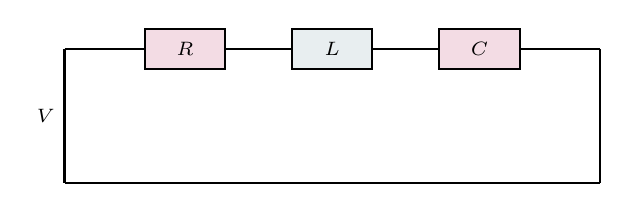
\begin{tikzpicture}[scale=0.85, every node/.style={font=\scriptsize}]
                \draw[thick] (0,0) -- (0,2);
                \draw[thick] (0,2) -- (1.2,2);
                \draw[thick,fill=cycfill] (1.2,1.7) rectangle (2.4,2.3)
                    node[midway]{$R$};
                \draw[thick] (2.4,2) -- (3.4,2);
                \draw[thick,fill=cycdofill] (3.4,1.7) rectangle (4.6,2.3)
                    node[midway]{$L$};
                \draw[thick] (4.6,2) -- (5.6,2);
                \draw[thick,fill=cycfill] (5.6,1.7) rectangle (6.8,2.3)
                    node[midway]{$C$};
                \draw[thick] (6.8,2) -- (8,2);
                \draw[thick] (8,2) -- (8,0);
                \draw[thick] (8,0) -- (0,0);
                \node[left] at (0,1) {$V$};
            \end{tikzpicture}
        \end{column}
    \end{columns}
\end{frame}

\begin{frame}[fragile]{Solving the Series Circuit in Python}
    \leavevmode
\begin{lstlisting}
import numpy as np

R, L, C, f = 40.0, 0.2, 50e-6, 60.0
omega = 2 * np.pi * f

Z_R = R
Z_L = 1j * omega * L
Z_C = -1j / (omega * C)

Z_total = Z_R + Z_L + Z_C   # series: impedances just add!

print(f"Total Impedance:   {Z_total.real:.1f} + {Z_total.imag:.2f}j Ohms")
print(f"Magnitude:         {np.abs(Z_total):.2f} Ohms")
print(f"Phase Angle:       {np.degrees(np.angle(Z_total)):.1f} degrees")
\end{lstlisting}
\end{frame}

\begin{frame}{Reading the Series Result}
    \leavevmode
    \texttt{Total Impedance: 40.0 + 22.35j Ohms} \\
    \texttt{Magnitude: 45.82 Ohms} \qquad
    \texttt{Phase Angle: 29.2 degrees}

    \vspace{4mm}
    \begin{block}{Interpret}
        Without a single trigonometry problem: the circuit opposes
        current with magnitude $45.82\,\Omega$, and current
        \alert{lags} voltage by $29.2^\circ$ --- a positive angle means
        \alert{inductive reactance dominates} at this frequency.
    \end{block}
\end{frame}

\begin{frame}{Visualizing Impedance on the Complex Plane}
    \leavevmode
    \begin{columns}[c]
        \begin{column}{.55\textwidth}
            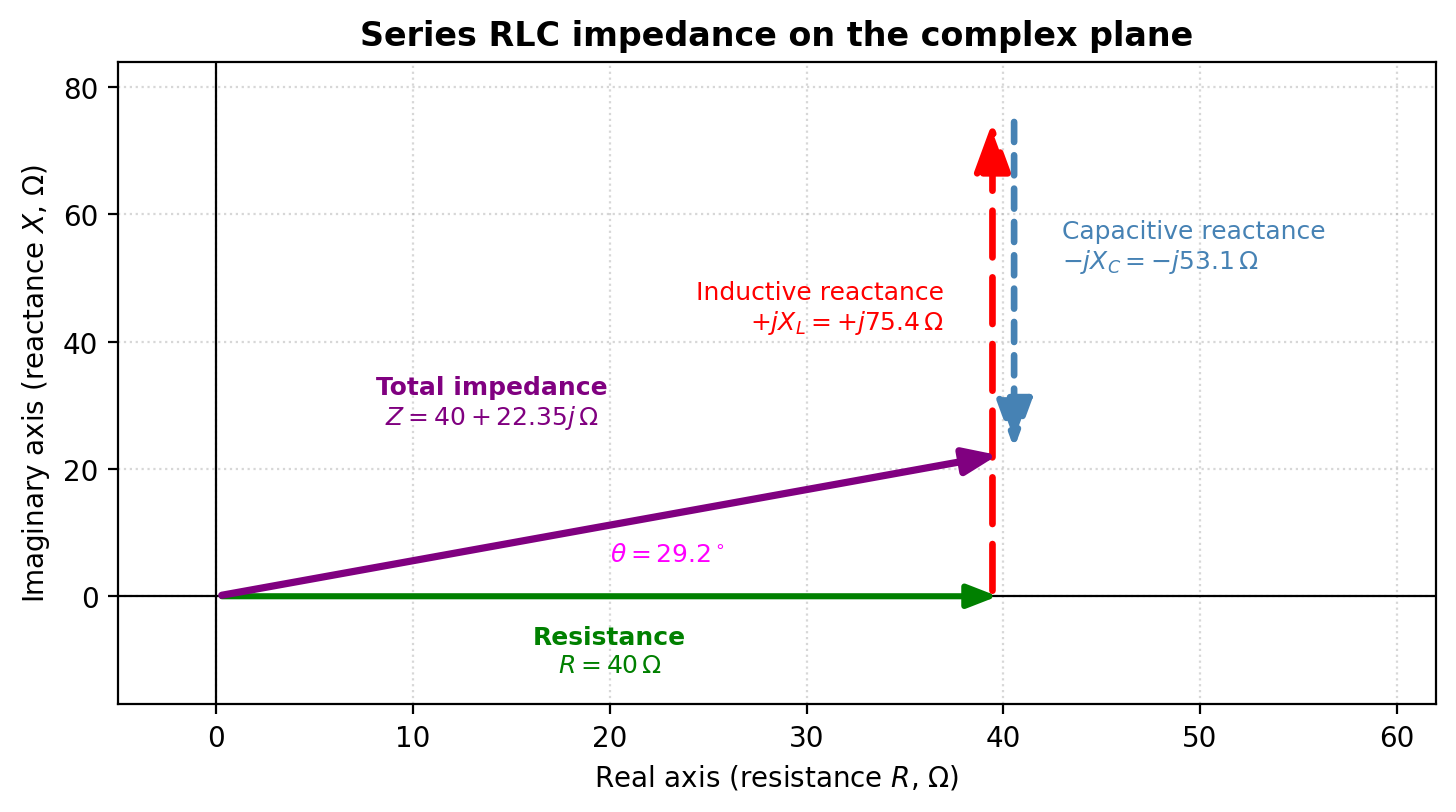
\includegraphics[width=\textwidth]{../images/chapter8/complex_impedance_phasor.png}
        \end{column}
        \begin{column}{.42\textwidth}
            \small
            Start at the origin: step $40\,\Omega$ right ($R$), step up
            $75.4\,\Omega$ ($+jX_L$), step down $53.1\,\Omega$
            ($-jX_C$).

            \vspace{2mm}
            The purple vector from origin to $40+22.35j$ is the total
            impedance $Z$: its \alert{length} is the magnitude, its
            \alert{angle} is the phase.
        \end{column}
    \end{columns}
\end{frame}

\begin{frame}{Inductors and Capacitors Cancel Each Other}
    \leavevmode
    The vector sum shows visually how inductors and capacitors actively
    oppose each other's effects.

    \vspace{3mm}
    \begin{alertblock}{A preview of resonance}
        If the frequency were tuned so that $X_L = X_C$, the upward and
        downward reactance steps would be exactly equal, and the total
        impedance would lie flat on the real axis.
    \end{alertblock}

    \vspace{2mm}
    {\small This fundamental electrical phenomenon is
    \alert{resonance} --- covered later in this chapter.}
\end{frame}

%===============================================================================
\section{Parallel RLC Circuits}
%===============================================================================

\begin{frame}{Parallel Impedances Combine as Reciprocals}
    \leavevmode
    In a series circuit the impedances add directly. In a
    \textbf{parallel} circuit they combine as reciprocals, exactly as
    parallel resistances do in DC:
    \[
    \frac{1}{Z_{\text{total}}} = \frac{1}{Z_R} + \frac{1}{Z_L} + \frac{1}{Z_C}.
    \]

    \vspace{3mm}
    \begin{block}{No manual algebra needed}
        This looks troublesome by hand --- rationalizing denominators,
        separating real and imaginary parts. Python's complex division
        handles it in \alert{one line}.
    \end{block}
\end{frame}

\begin{frame}[fragile]{Same Components, Connected in Parallel}
    \leavevmode
\begin{lstlisting}
import numpy as np

R, L, C, f = 40.0, 0.2, 50e-6, 60.0
omega = 2 * np.pi * f

Z_R = R
Z_L = 1j * omega * L
Z_C = -1j / (omega * C)

# Parallel combination: reciprocal of the sum of reciprocals
Z_total = 1 / (1/Z_R + 1/Z_L + 1/Z_C)

print(f"Z_total = {Z_total.real:.2f} + {Z_total.imag:.2f}j Ohms")
print(f"Magnitude: {np.abs(Z_total):.2f} Ohms")
print(f"Phase angle: {np.degrees(np.angle(Z_total)):.2f} degrees")
\end{lstlisting}
\end{frame}

\begin{frame}{Topology Matters as Much as Component Values}
    \leavevmode
    \texttt{Z\_total = 38.10 + -8.51j Ohms} \quad
    \texttt{Magnitude: 39.04} \quad
    \texttt{Phase: -12.60\textdegree}

    \vspace{4mm}
    \begin{columns}[t]
        \begin{column}{.5\textwidth}
            \begin{block}{Series (same parts)}
                \small $40 + 22.35j\,\Omega$, magnitude $45.82\,\Omega$,
                phase $+29.2^\circ$ --- net \alert{inductive}.
            \end{block}
        \end{column}
        \begin{column}{.5\textwidth}
            \begin{alertblock}{Parallel (same parts)}
                \small $38.10 - 8.51j\,\Omega$, magnitude
                $39.04\,\Omega$, phase $-12.6^\circ$ --- net
                \alert{capacitive}.
            \end{alertblock}
        \end{column}
    \end{columns}

    \vspace{3mm}
    {\small Same three components. Different connection. Opposite
    character.}
\end{frame}

%===============================================================================
\section{Power in AC Circuits}
%===============================================================================

\begin{frame}{$P = VI$ Is Wrong for AC}
    \leavevmode
    In DC, power is simply $P = VI$. In AC, that formula fails whenever
    the load is not purely resistive --- voltage and current no longer
    peak at the same instant.

    \vspace{3mm}
    Three separate quantities are needed, and confusing them is a
    classic error:
    \begin{itemize}
        \item \textbf{Real power} $P$ (W) --- actually converted to
              heat or work. The only part the meter charges for.
        \item \textbf{Reactive power} $Q$ (VAR) --- sloshes back and
              forth, doing no net work.
        \item \textbf{Apparent power} $S$ (VA) --- what the cabling
              must be sized to carry.
    \end{itemize}
\end{frame}

\begin{frame}{The Power Triangle and Power Factor}
    \leavevmode
    \[
    S = \sqrt{P^{2} + Q^{2}}, \qquad P = S\cos\theta, \qquad Q = S\sin\theta.
    \]

    \vspace{2mm}
    \[
    \text{power factor} = \cos\theta = \frac{P}{S}.
    \]

    \vspace{3mm}
    \begin{block}{What power factor tells you}
        What fraction of delivered capacity does useful work. Purely
        resistive: $\cos\theta = 1$. Purely reactive: $\cos\theta = 0$
        --- no work at all.
    \end{block}
\end{frame}

\begin{frame}[fragile]{Complex Power: $S = VI^{*}$}
    \leavevmode
\begin{lstlisting}
import numpy as np

R, L, C, f = 40.0, 0.2, 50e-6, 60.0
V = 120.0                          # supply voltage (RMS)

omega = 2 * np.pi * f
Z = R + 1j*omega*L - 1j/(omega*C)

I = V / Z                          # complex current (Ohm's law)
S = V * np.conj(I)                 # complex power

print(f"Real power P:      {S.real:.2f} W")
print(f"Reactive power Q:  {S.imag:.2f} VAR")
print(f"Apparent power S:  {np.abs(S):.2f} VA")
print(f"Power factor:      {np.cos(np.angle(Z)):.4f}")
\end{lstlisting}
\end{frame}

\begin{frame}{Checking and Interpreting the Power Result}
    \leavevmode
    \texttt{P: 274.37 W} \quad \texttt{Q: 153.28 VAR} \quad
    \texttt{S: 314.28 VA} \quad \texttt{PF: 0.8730}

    \vspace{3mm}
    \begin{block}{Check}
        \small $P$ must equal $|I|^2 R = 2.619^2 \times 40 = 274.4\,$W
        --- it does. And $\sqrt{P^2+Q^2} = 314.3\,$VA matches $S$.
    \end{block}

    \vspace{2mm}
    \begin{alertblock}{Interpret}
        \small Only $274\,$W of the $314\,$VA supplied does useful
        work. Industrial customers are penalised for poor power
        factor --- capacitors are added alongside motors to cancel
        inductive $Q$ and pull $\cos\theta$ toward unity.
    \end{alertblock}
\end{frame}

%===============================================================================
\section{Resonance}
%===============================================================================

\begin{frame}{When Reactances Cancel Exactly}
    \leavevmode
    $X_L = \omega L$ grows with frequency; $X_C = 1/\omega C$ shrinks.
    At some frequency the two must be equal.

    \vspace{3mm}
    \begin{block}{Resonant frequency}
        \[
        \omega_0 L = \frac{1}{\omega_0 C} \quad\Longrightarrow\quad
        f_0 = \frac{1}{2\pi\sqrt{LC}}.
        \]
    \end{block}

    \vspace{2mm}
    \begin{alertblock}{At resonance}
        The imaginary part of $Z$ vanishes: $Z = R$. The circuit
        behaves as though the inductor and capacitor were not there.
    \end{alertblock}
\end{frame}

\begin{frame}[fragile]{Finding Resonance in Python}
    \leavevmode
\begin{lstlisting}
import numpy as np

R, L, C, V = 40.0, 0.2, 50e-6, 120.0

f0 = 1 / (2*np.pi*np.sqrt(L*C))
omega0 = 2*np.pi*f0

X_L = omega0 * L
X_C = 1 / (omega0 * C)
Z0  = R + 1j*X_L - 1j*X_C

print(f"Resonant frequency: {f0:.2f} Hz")
print(f"Z at resonance:     {Z0.real:.1f} + {Z0.imag:.4f}j Ohms")
print(f"Current at f0:      {np.abs(V/Z0):.3f} A")
\end{lstlisting}
\end{frame}

\begin{frame}{Three Consequences of Resonance}
    \leavevmode
    \texttt{f0 = 50.33 Hz} \quad \texttt{Z = 40.0 + 0.0000j} \quad
    \texttt{Current = 3.000 A}

    \vspace{3mm}
    \begin{itemize}
        \item \textbf{Current peaks.} Impedance is smallest, so a
              modest voltage drives a large current --- exploited in
              radio tuning, dangerous in power systems.
        \item \textbf{Power factor becomes unity.} $\theta = 0$,
              $\cos\theta = 1$: every VA does useful work.
        \item \textbf{Character flips with frequency.} Below $f_0$:
              capacitive, current leads. Above $f_0$: inductive,
              current lags.
    \end{itemize}

    \vspace{2mm}
    {\small Check: the two reactances agree to three decimals, but $Z$'s
    imaginary part is never exactly zero in floating point --- a reason
    to avoid testing with \texttt{==}.}
\end{frame}

\begin{frame}{Sweeping Frequency: The Resonance Dip}
    \leavevmode
    \begin{center}
    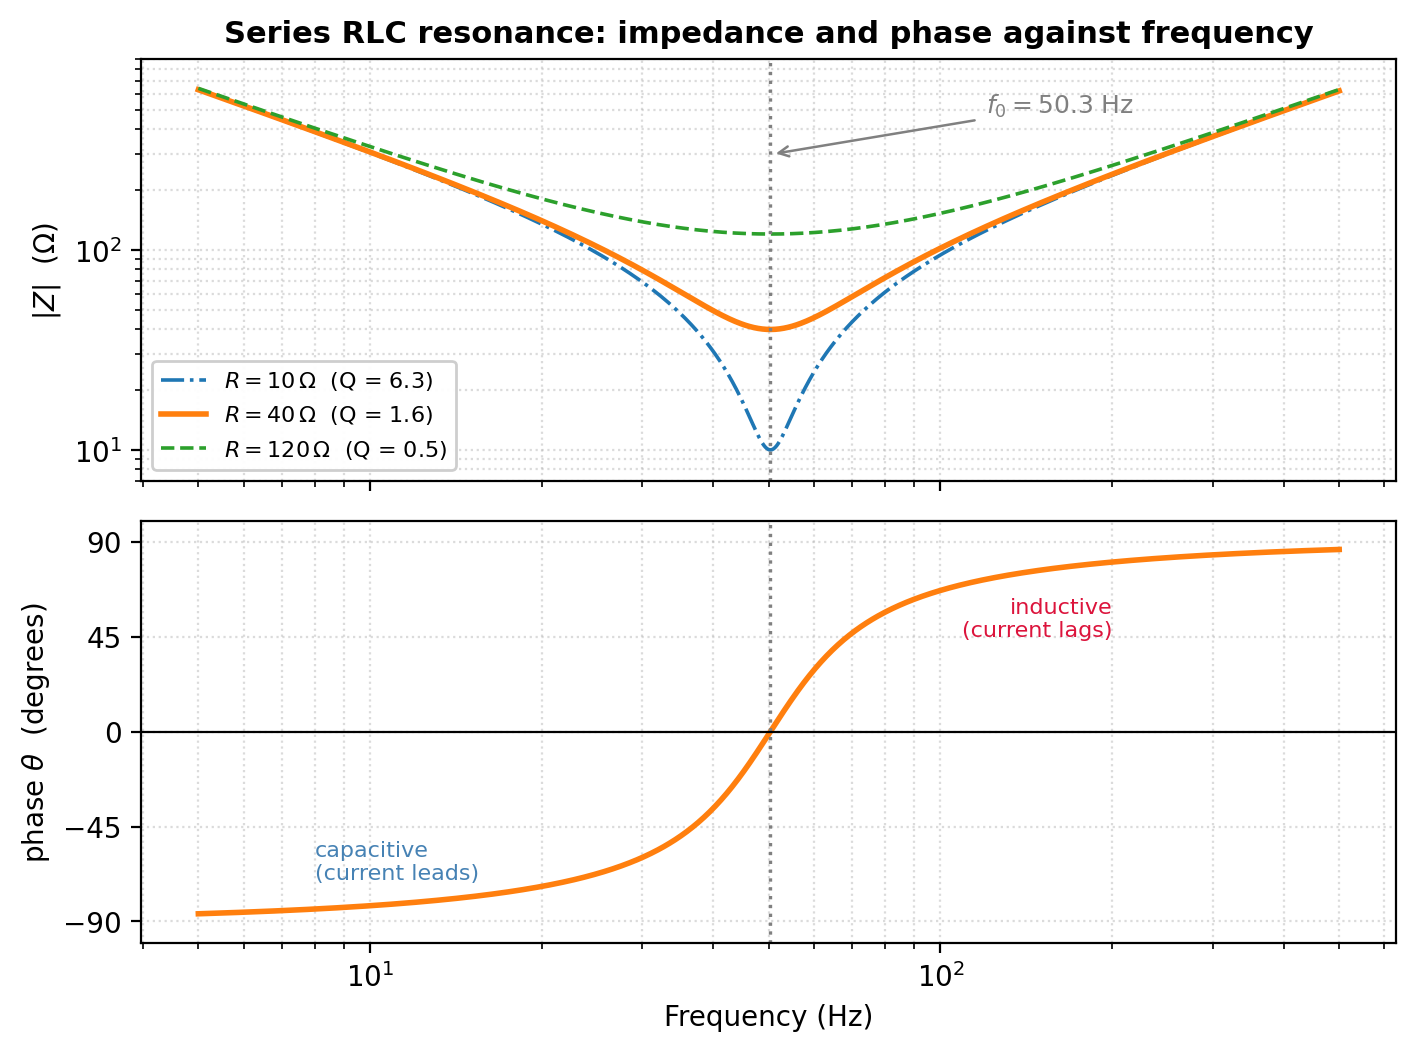
\includegraphics[height=0.64\textheight]{../images/chapter8/resonance_sweep.png}
    \end{center}

    {\scriptsize Both axes logarithmic. The minimum sits at $f_0$ for
    every curve --- changing $R$ moves the dip up or down, never
    sideways.}
\end{frame}

\begin{frame}{The Quality Factor}
    \leavevmode
    How sharp the resonance dip is depends on resistance:
    \[
    Q_{\text{factor}} = \frac{1}{R}\sqrt{\frac{L}{C}}.
    \]

    \vspace{3mm}
    \begin{columns}[t]
        \begin{column}{.5\textwidth}
            \begin{block}{Low $R$ ($10\,\Omega$)}
                \small Deep, narrow dip. Strong but selective response
                --- good for tuning a radio to one station.
            \end{block}
        \end{column}
        \begin{column}{.5\textwidth}
            \begin{alertblock}{High $R$ ($120\,\Omega$)}
                \small Shallow, broad dip. Still resonates, but barely
                distinguishes $f_0$ from its neighbours.
            \end{alertblock}
        \end{column}
    \end{columns}

    \vspace{3mm}
    {\scriptsize This $Q$ (dimensionless sharpness) is unrelated to the
    reactive power $Q$ from the previous section --- an unfortunate
    clash of notation in electrical engineering.}
\end{frame}

%===============================================================================
\section{Summary}
%===============================================================================

\begin{frame}{What This Chapter Covered}
    \leavevmode
    \small
    \begin{itemize}
        \item Python writes complex numbers with a \texttt{j} suffix
              (\texttt{3 + 4j}); must be \texttt{1j}, never bare
              \texttt{j}.
        \item \textbf{Rectangular} suits $+/-$; \textbf{polar} suits
              $\times/\div$. \texttt{abs()} and \texttt{np.angle()}
              convert between them.
        \item \textbf{Impedance} $Z = R + jX$ generalises resistance;
              $X_L = \omega L$ (positive), $X_C = -1/\omega C$
              (negative).
        \item Series impedances \alert{add}; parallel impedances
              combine by \alert{reciprocal} --- same rule as DC
              resistors, complex arithmetic.
        \item \textbf{Magnitude} sets current flow; \textbf{phase}
              says whether the load is capacitive or inductive.
        \item AC power splits into $P$ (W), $Q$ (VAR), $S$ (VA), with
              $S = \sqrt{P^2+Q^2}$ and complex power $S = VI^{*}$.
        \item \textbf{Power factor} $\cos\theta = P/S$; correcting it
              (adding capacitance to inductive loads) reduces current
              for the same real power.
        \item At \textbf{resonance}, $f_0 = 1/(2\pi\sqrt{LC})$,
              reactances cancel, $Z=R$, current peaks, power factor
              hits unity.
        \item \textbf{Quality factor} $(1/R)\sqrt{L/C}$ measures how
              sharply a circuit selects its resonant frequency.
    \end{itemize}
\end{frame}

\begin{frame}{Where This Is Going}
    \leavevmode
    \small
    This chapter turned AC circuit analysis into ordinary algebra with
    complex numbers. The next chapter extends this to circuits with
    \alert{multiple} loops and nodes.

    \vspace{3mm}
    \begin{itemize}
        \item Chapter 9: Matrices and Circuit Equations ---
              representing a whole circuit as $A\mathbf{x} = \mathbf{b}$
              and solving it in one line.
        \item The complex-number skills here carry over directly: AC
              mesh equations are solved with the same \texttt{numpy}
              linear algebra, just with complex entries.
    \end{itemize}

    \vspace{4mm}
    \begin{center}
        \large\color{primary}\textbf{Next: Matrices and Circuit Equations}
    \end{center}
\end{frame}

\end{document}
